\chapter{Конструкторская часть}

В данном разделе будут представлены схемы муравьиного алгоритма, алгоритма полного перебора
и вспомогательного алгоритма выбора следующего города.

\section{Схемы алгоритмов}

Схема реализации муравьиного алгоритма без элитных муравьев для решения задачи коммивояжёра представлена на рисунках~\ref{fig:schema_num1_part1}---\ref{fig:schema_num1_part2}.




Схема алгоритма выбора следующего города приведена на рисунке~\ref{fig:schema_num2}. 

Схема алгоритма полного перебора приведена на рисунке~\ref{fig:schema_num4}.

\begin{figure}[h!]
	\centering
	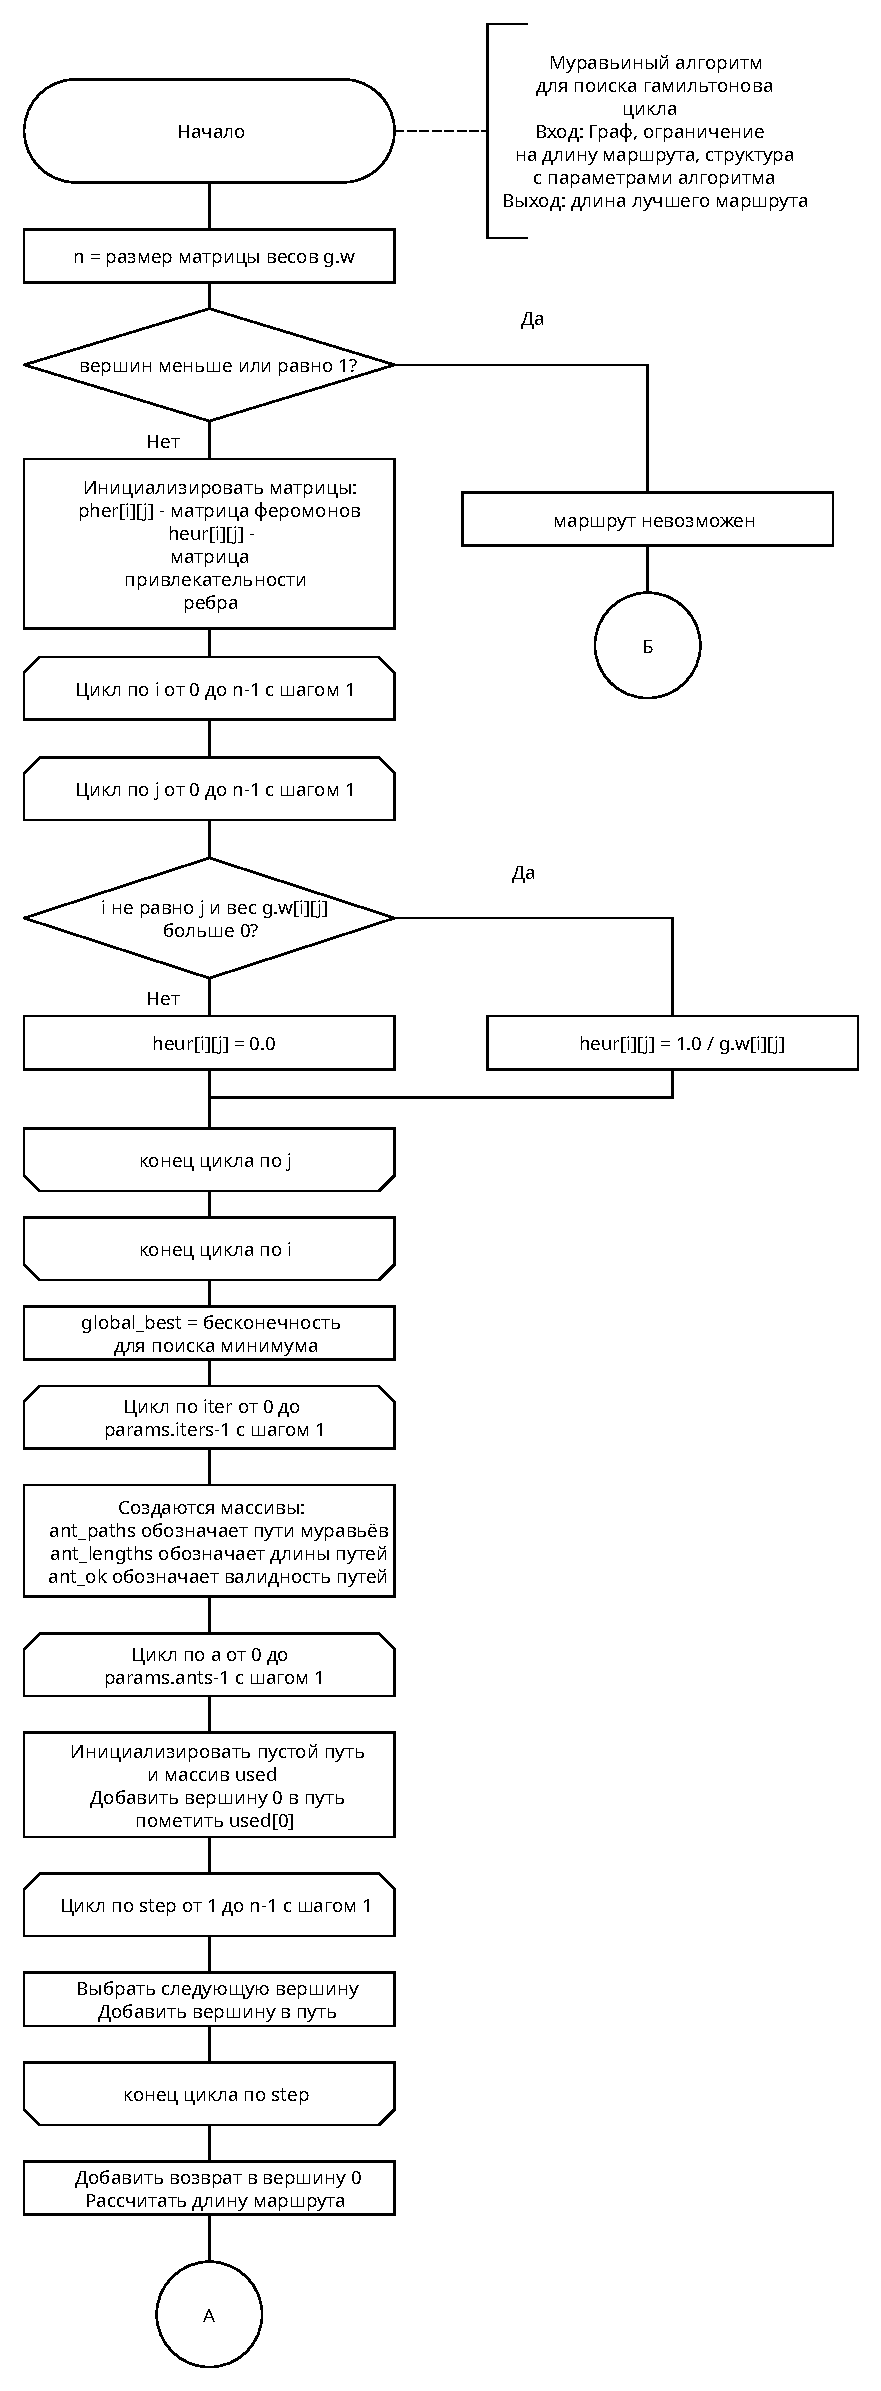
\includegraphics[width=0.55\textwidth]{images/schema_num1_part1.pdf}
	\caption{Схема алгоритма решения задачи коммивояжёра часть 1}
	\label{fig:schema_num1_part1}
\end{figure}

\clearpage

\begin{figure}[h!]
	\centering
	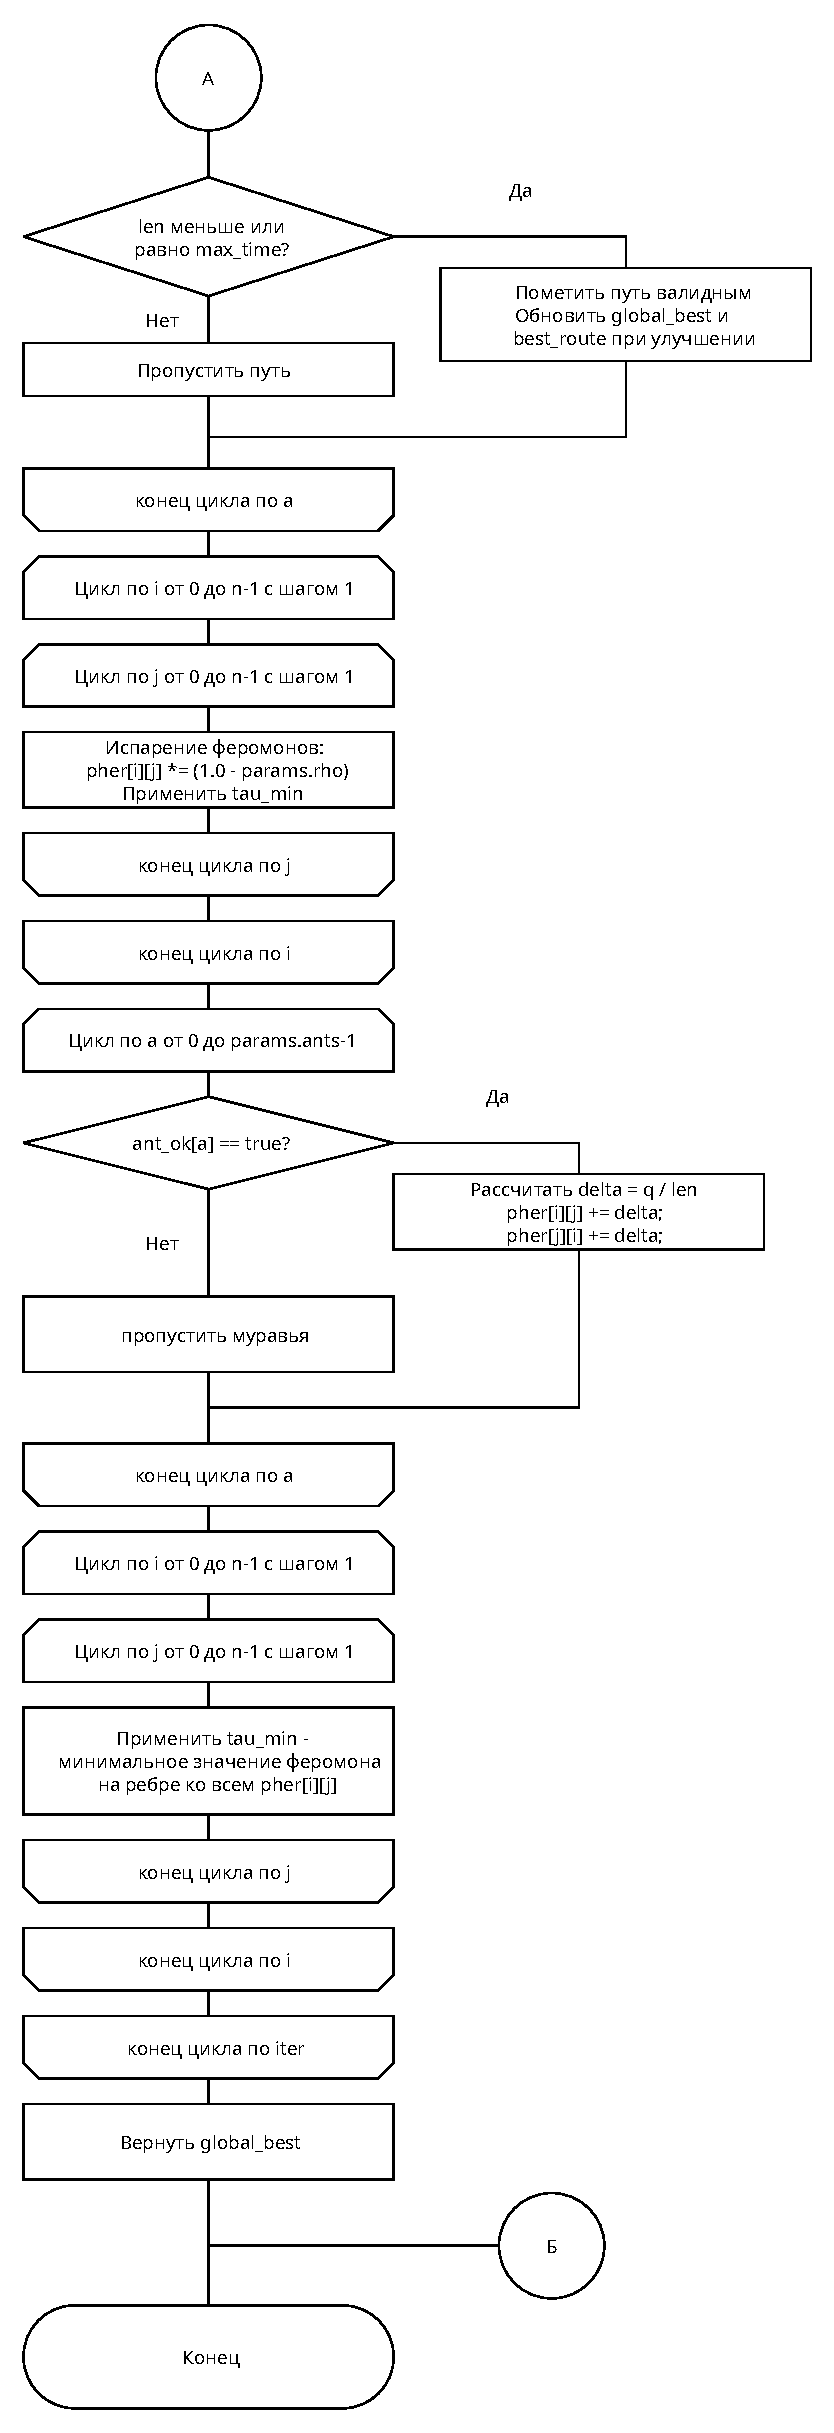
\includegraphics[width=0.47\textwidth]{images/schema_num1_part2.pdf}
	\caption{Схема алгоритма решения задачи коммивояжёра часть 2}
	\label{fig:schema_num1_part2}
\end{figure}

\clearpage
 
\begin{figure}[h!]
	\centering
	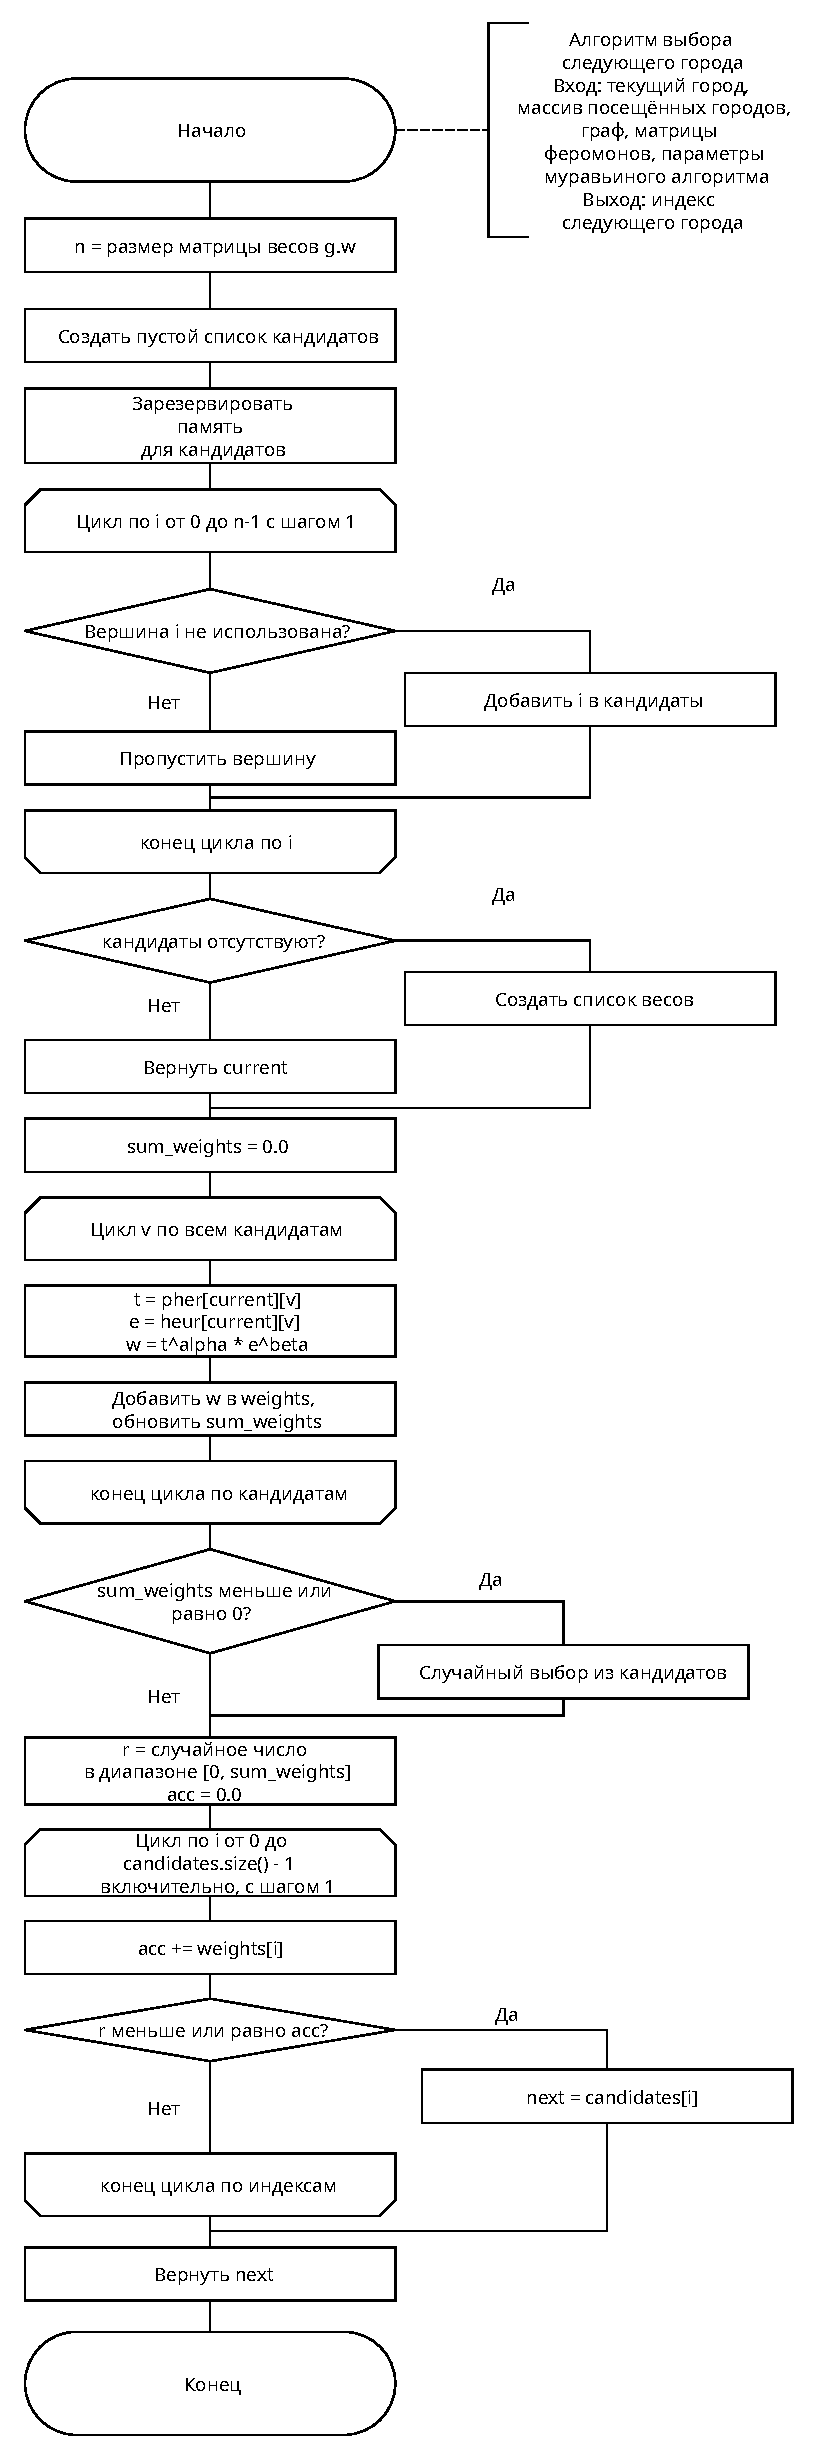
\includegraphics[width=0.5\textwidth]{images/schema_num2.pdf}
	\caption{Схема алгоритма выбора следующего города}
	\label{fig:schema_num2}
\end{figure}

\clearpage


\begin{figure}[h!]
	\centering
	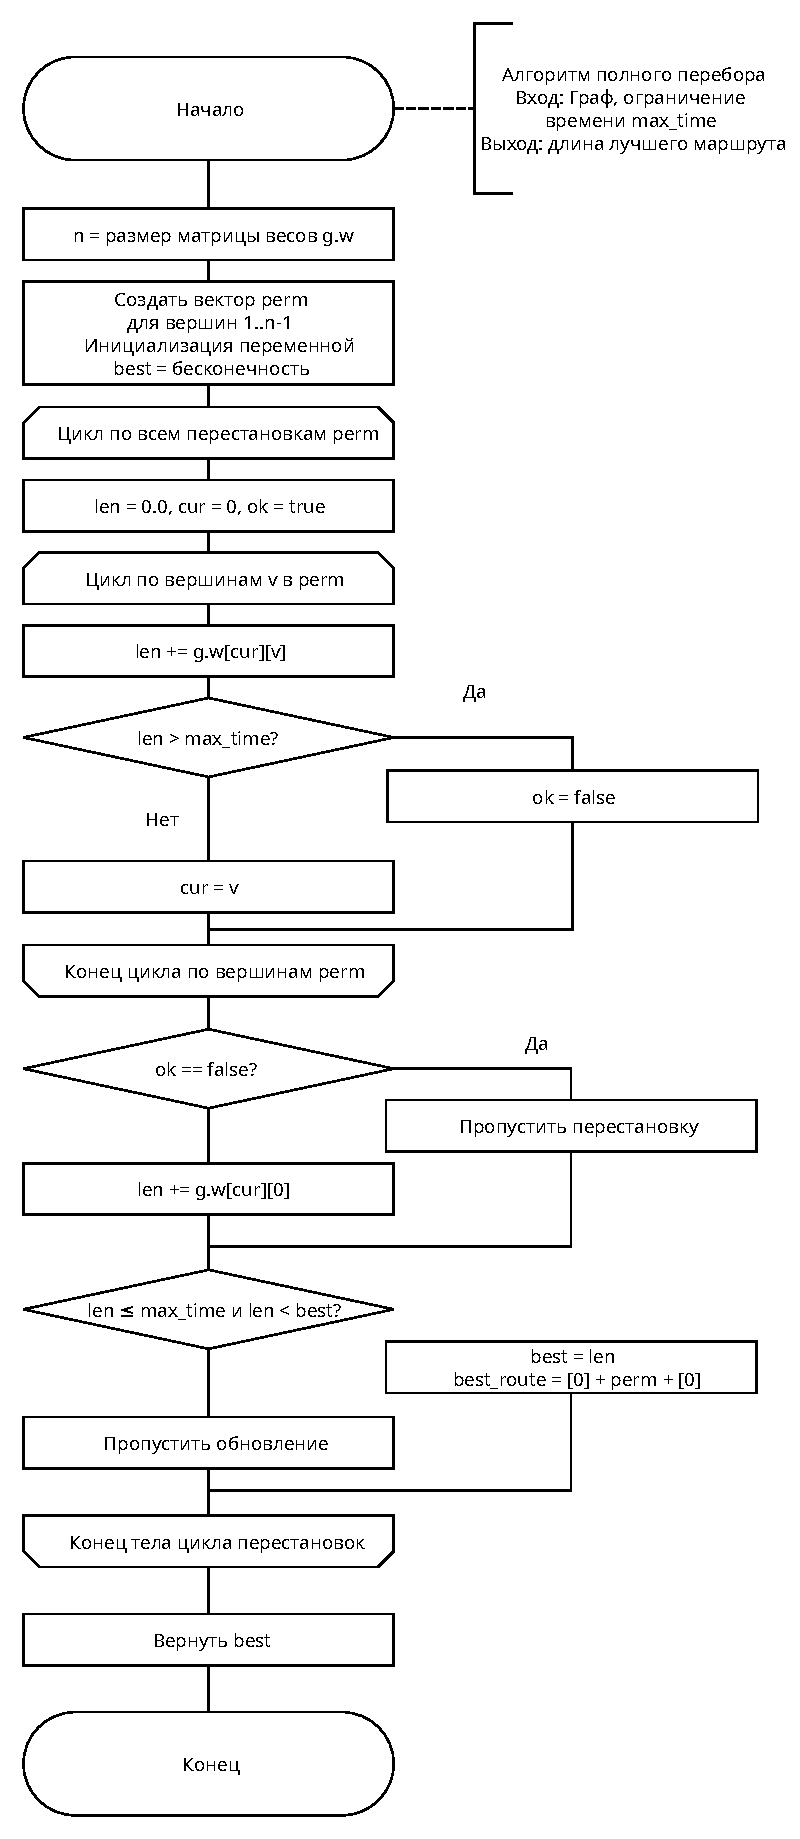
\includegraphics[width=0.5\textwidth]{images/schema_num4.pdf}
	\caption{Схема алгоритма полного перебора}
	\label{fig:schema_num4}
\end{figure}

\clearpage

\section{Трудоёмкости алгоритмов}

\subsection{Модель вычислений}

Для последующего вычисления трудоёмкости необходимо ввести модель вычислений:

\begin{enumerate}
	\item операции из списка (\ref{eq:operations}) имеют трудоёмкость 1;
	
	\begin{equation}
		\label{eq:operations}
		+, -, =, ==, !=, <, >, <=, >=, [], ++, {-}-, +=, -=, \text{<<}, \text{>>}
	\end{equation}
	
	\item операции умножения, деления и взятия остатка имеют трудоёмкость 2;
	
	\item трудоёмкость условного оператора \textbf{if} рассчитывается по формуле (\ref{eq:if});
	
	\begin{equation}
		\label{eq:if}
		f_{if} = f_{\text{условия}} +
		\begin{cases}
			f_A, & \text{если условие выполняется}, \\
			f_B, & \text{иначе}.
		\end{cases}
	\end{equation}
	
	\item трудоёмкость цикла рассчитывается как~(\ref{eq:for});
	
	\begin{equation}
		\label{eq:for}
		f_{for} = f_{\text{инициализации}} + f_{\text{сравнения}} + N(f_{\text{тела}} + f_{\text{инкремента}} + f_{\text{сравнения}})
	\end{equation}
	
	\item трудоёмкость вызова функции и возврата результата равна 0;
	
\end{enumerate}

В следующих частях будут рассчитаны трудоёмкости алгоритмов поиска гамильтонова цикла минимальной длины с ограничением по времени.

Для расчёта трудоёмкости используются следующие обозначения:
\begin{itemize}
	\item $n$ --- количество вершин в графе;
	\item $m = n-1$ --- количество вершин без учёта стартовой;
	\item $A$ --- количество муравьёв в алгоритме;
	\item $I$ --- количество итераций муравьиного алгоритма;
	\item $\alpha$ --- константа перехода к следующей перестановке.
\end{itemize}

\subsection{Алгоритм полного перебора}

Трудоёмкость алгоритма полного перебора состоит из:

\begin{itemize}
	\item генерации всех перестановок $m$ вершин, количество которых равно:~(\ref{eq:perm_count})
	
	\begin{equation}
		\label{eq:perm_count}
		P = m!
	\end{equation}
	
	\item проверки каждого маршрута, которая включает:
	\begin{itemize}
		\item инициализацию ($f_{\text{init}} = 3$);
		\item проверку $m$ рёбер в перестановке;
		\item проверку последнего ребра к стартовой вершине ($f_{\text{last}} = 3$);
	\end{itemize}
	
	\item трудоёмкости проверки одного ребра ($f_{\text{edge}}$):
	\begin{itemize}
		\item обращение к матрице весов: 1;
		\item сложение: 1;
		\item сравнение с максимальным временем: 1;
		\item условный переход: 1 (в худшем случае);
	\end{itemize}
	
	Таким образом, $f_{\text{edge}} = 4$.
\end{itemize}

Трудоёмкость проверки одного маршрута:~(\ref{eq:route_cost})

\begin{equation}
	\label{eq:route_cost}
	f_{\text{route}} = 3 + 4m + 3 = 4m + 6
\end{equation}

Трудоёмкость перехода к следующей перестановке составляет $\alpha m$.

Итоговая трудоёмкость алгоритма полного перебора:~\ref{eq:brute_total}

\begin{equation}
	\label{eq:brute_total}
	f_{\text{brute}}(n) = P \cdot (f_{\text{route}} + \alpha m) = m! \cdot (4m + 6 + \alpha m)
\end{equation}

Доминирующий член:~(\ref{eq:brute_dominant})

\begin{equation}
	\label{eq:brute_dominant}
	f_{\text{brute}}(n) = \Theta(m! \cdot m) = \Theta((n-1)! \cdot (n-1)) = \Theta(n!)
\end{equation}

\subsection{Муравьиный алгоритм}

Трудоёмкость муравьиного алгоритма складывается из построения маршрутов всеми муравьями и обновления феромонов.

\subsubsection{Построение маршрута одним муравьём}

Трудоёмкость функции алгоритма выбора следующего города:

\begin{itemize}
	\item создание вектора кандидатов: $2 + n \cdot 4 = 4n + 2$;
	\item вычисление весов: $2 + n \cdot 16 = 16n + 2$;
	\item выбор следующей вершины: $2 + 4n = 4n + 2$;
\end{itemize}

\begin{equation}
	\label{eq:choose_cost}
	f_{\text{choose}} = (4n + 2) + (16n + 2) + (4n + 2) = 24n + 6
\end{equation}

Трудоёмкость построения маршрута одним муравьём:~(\ref{eq:build_one})

\begin{equation}
	\label{eq:build_one}
	f_{\text{build\_ant}} = 5 + m \cdot f_{\text{choose}} + 2n + 3 = 5 + (n-1)(24n+6) + 2n + 3
\end{equation}

Упрощая:~(\ref{eq:build_one_simple})

\begin{equation}
	\label{eq:build_one_simple}
	f_{\text{build\_ant}} = 24n^2 - 16n + 8
\end{equation}

\subsubsection{Обновление феромонов}

Трудоёмкость испарения феромонов:~(\ref{eq:evap_cost})

\begin{equation}
	\label{eq:evap_cost}
	f_{\text{evap}} = 2 + n \cdot \bigl(2 + n \cdot (2 + 4)\bigr) = 2 + 2n + 6n^2
\end{equation}

Трудоёмкость добавления феромона для одного маршрута длины $n+1$:~(\ref{eq:add_route})

\begin{equation}
	\label{eq:add_route}
	f_{\text{add\_route}} = 4 + (n+1) \cdot 10 = 10n + 14
\end{equation}

Трудоёмкость обновления феромонов для всех маршрутов ($A_{\text{ok}}$ --- число успешных маршрутов):~(\ref{eq:update_all})

\begin{equation}
	\label{eq:update_all}
	f_{\text{update}} = f_{\text{evap}} + A_{\text{ok}} \cdot f_{\text{add\_route}} + 2
\end{equation}

\subsubsection{Трудоёмкость одной итерации}

Трудоёмкость одной итерации муравьиного алгоритма:~(\ref{eq:iter_cost})

\begin{equation}
	\label{eq:iter_cost}
	f_{\text{iter}} = A \cdot f_{\text{build\_ant}} + f_{\text{update}} + 4
\end{equation}

Подставляя формулы (\ref{eq:build_one_simple}) и (\ref{eq:update_all}):

\begin{equation}
	\label{eq:iter_full}
	f_{\text{iter}} = A(24n^2 - 16n + 8) + (2 + 2n + 6n^2) + A_{\text{ok}}(10n + 14) + 6
\end{equation}

\subsubsection{Общая трудоёмкость алгоритма}

Общая трудоёмкость муравьиного алгоритма:~(\ref{eq:ant_total})

\begin{equation}
	\label{eq:ant_total}
	f_{\text{ant}}(n, A, I) = I \cdot f_{\text{iter}}
\end{equation}

Подставляя формулу~(\ref{eq:iter_full}):

\begin{equation}
	f_{\text{ant}} = I \cdot \bigl(A(24n^2 - 16n + 8) + 2 + 2n + 6n^2 + A_{\text{ok}}(10n + 14) + 6\bigr)
	\label{eq:ant_full}
\end{equation}

Упрощённая оценка (в худшем случае, когда все маршруты успешны: $A_{\text{ok}} = A$):

\begin{equation}
	\label{eq:ant_simple}
	f_{\text{ant}}(n, A, I) = O(I \cdot A \cdot n^2)
\end{equation}

\subsection{Сравнение алгоритмов}

Сравнительный анализ временной сложности алгоритмов показывает:

\begin{itemize}
	\item \textbf{алгоритм полного перебора}: $\Theta(n!)$
	\item \textbf{муравьиный алгоритм}: $O(I \cdot A \cdot n^2)$
\end{itemize}

где:
\begin{itemize}
	\item $n$ --- количество вершин графа,
	\item $I$ --- количество итераций муравьиного алгоритма,
	\item $A$ --- количество муравьёв в колонии.
\end{itemize}

Муравьиный алгоритм имеет полиномиальную трудоёмкость при фиксированных параметрах $I$ и $A$, что делает его применимым для сложных задач, по сравнению с полным перебором, имеющим факториальную сложность.

\section*{Вывод}

В данном разделе были представлены схемы алгоритмов полного перебора и муравьиного алгоритма для решения задачи коммивояжёра с ограничением по времени. Проведён анализ трудоёмкости.

\clearpage
